\chapter{Working context}\label{chap:organisation}

In this chapter, we will discover how I accomplished my work within the Intel Audio team.
This includes developer process, planning schedule and agile methodology.

\section{Workflow and environment}
In this section, we will cover my daily workflow. This helps
to understand the routine I had during my whole internship.

Figure \ref{fig:workflow} below shows the development process I used during my internship.
It is a strict procedure that results in software of great quality with very few defects.

\begin{figureGraphics}{Developer workflow}{fig:workflow}
    \includegraphics[height=0.6\textheight]{./src/img/workflow.pdf}
\end{figureGraphics}

This workflow is the same for every developer of the Intel Audio team. It is
detailed in the subsections below.

\subsection{Development}
Android source tree contains more than 700 projects. They have their own build system
based on \lstinline{Android.mk} files. Each time that a project has to be rebuild from scratch (for example after a  \lstinline{make clean} command) all
the 700 projects of the Android source tree are scanned for dependencies. This requires a lot of computing power.
Given that fact, most of developers of our team are working on a remote server, via ssh.
The server we are connecting to is far more powerful than the desktops we use.
With its 32 cores and its 2 TeraBytes of SSD, compilation time was far less time-consuming
than compiling on my local machine (about 10 times faster).
This server also helps to have the same developer environment to avoid
time-consuming installations on local machines.

Working remotely on that server restrict developers to use command line programs only because
launching a graphical session for each user would require too much computing power.
During my internship, I sharpened my skills in \gls{vim} and discovered \gls{tmux}.
On the figure \ref{fig:setup} below, there is a screenshot of my development setup at Intel.

\begin{figureGraphics}{Development setup with vim and tmux}{fig:setup}
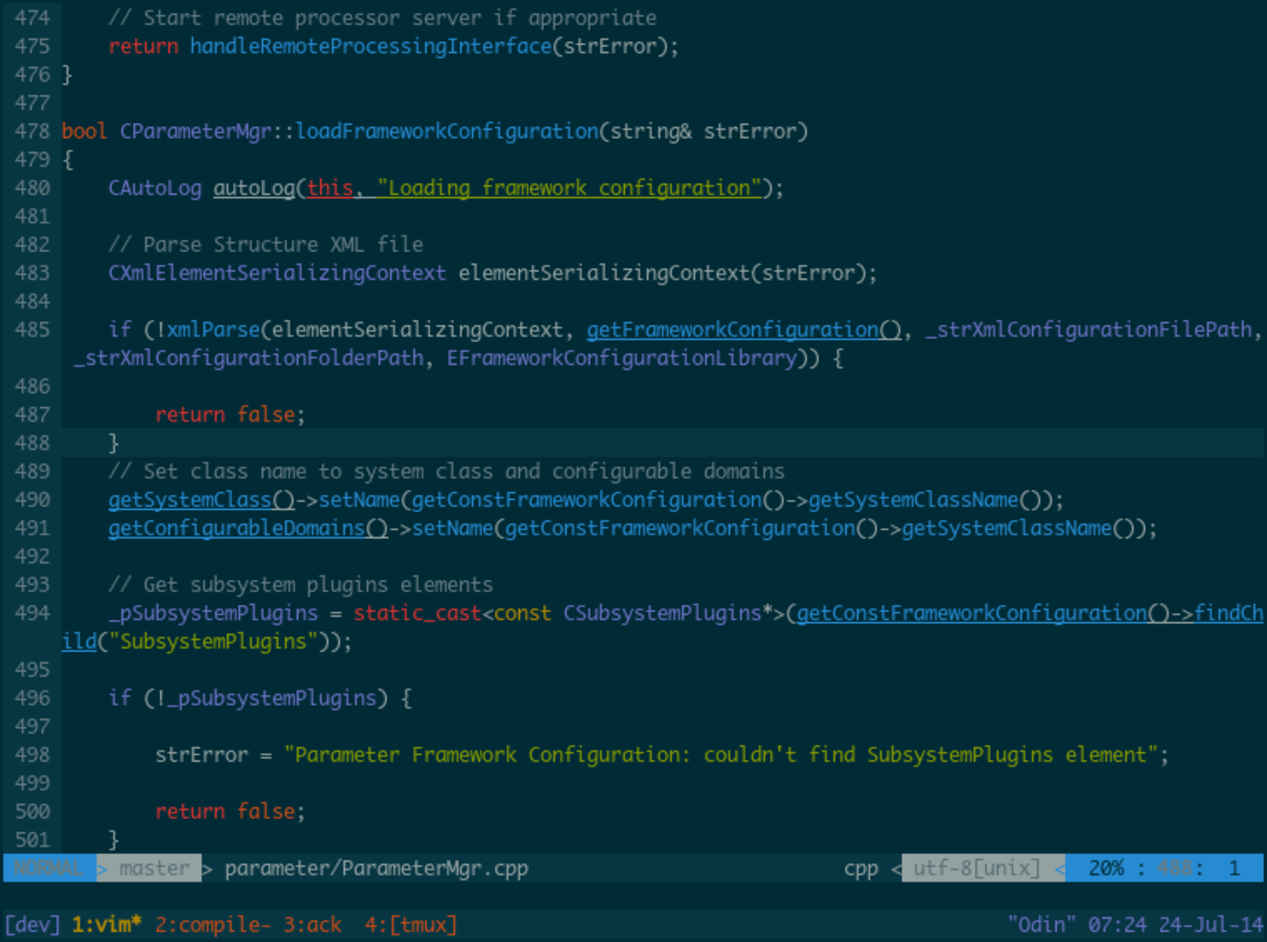
\includegraphics[width=\textwidth]{./src/img/setup.pdf}
\end{figureGraphics}

When the code is ready, I push it via \gls{git} on \gls{gerrit} to be reviewed.

\subsection{Git}
\gls{git} is a distributed revision control system initially designed for kernel
development. Given that fact, it can be used in environment which have large
code bases, such as \gls{android}. We use \gls{git} on daily basis at Intel for the
code delivered to customers and for the internal tools.

\subsection{Code quality}
Code quality matters. Clean code eases maintenance and is less error-prone.
Those facts are driving the team that I worked with at Intel. Naturally, all the
patches I have delivered during my internship have been reviewed and met the
expected quality.

Those reviews are done with the official \gls{android} review tool which is \gls{gerrit}.
It is based on a notation system with inline comments and its usage is pretty straightforward.
Its interface is showed on figure \ref{fig:gerrit} below.

\begin{figureGraphics}{Gerrit code review}{fig:gerrit}
    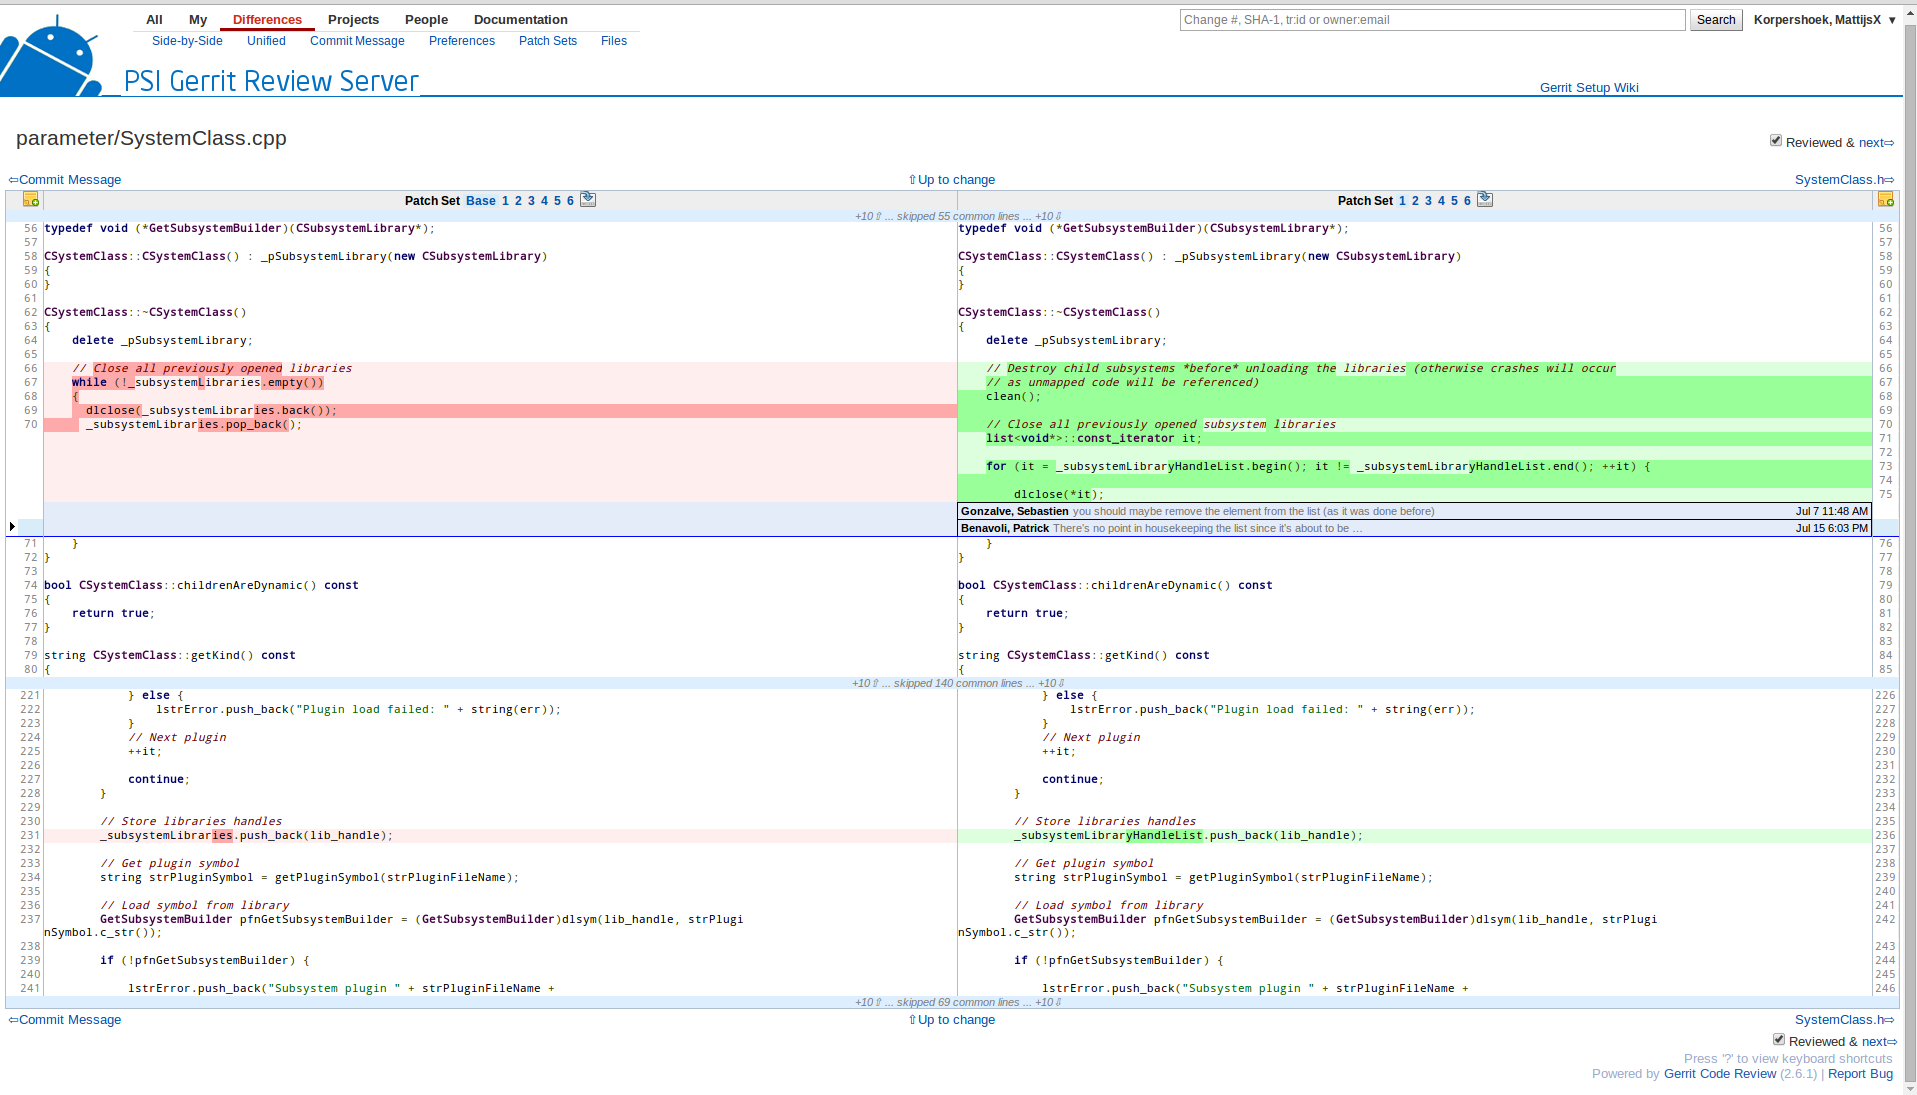
\includegraphics[width=\textwidth]{./src/img/gerrit.png}
\end{figureGraphics}

I have done some code review myself during this internship. It helps a lot to
understand how other people work. Viewing other peoples code also makes me come
up with new ideas to improve my own work in several aspects such as better naming,
more modularity, cleaner design.

\subsection{Submission to gatekeeping team}
After code review and a few reworks, the code is validated by the development team.
The super reviewer gives the developer the permission to submit his work to the gatekeeping team.
They are responsible for testing complex use cases and they ensure there is no regression nor side effects
due to the modifications the development team made.
A lot of automatic and manual tests scenarios are ran which cover \emph{voice call}, \emph{voip call}, \emph{media playback}
and more. Of course, more complex tests are done depending on the functionality which is developed.



\section{Planning}
\subsection{Discovering the code}
During the first work week, I dug into the Parameter-framework's code. I had no
documentation at all, just the code on \gls{GitHub}. The absence of help was done on
purpose: the team needed an external point of view on the source code. I had
to understand the powerful concepts of the Parameter-framework just by reading
the code. Since I struggled a bit with the concepts, I decided to write some
newcomer tutorials which content is described at section \ref{sec:tutorials}.
I started to submit code quite early (the second week), with \gls{pullrequests} on \gls{GitHub}.

\subsection{Joining forces with the scrum team}
After three weeks, I requested to join a \gls{scrum} team so that I could experience
Intel's way of working with \gls{scrum}!
For the rest of my internship I was an \emph{agile developer} just like the other members of the team.
In section \ref{sec:agile}, I describe a bit more agile methodology and the contributions I made to improve
the \gls{scrum} process.

\subsection{Gantt chart}
Since we are working agile, I did not had a detailed planning at the begin of my internship.
I had two leading directions which were about open-sourcing the \gls{pfw} and delivering new features
to Intel's customers.
This Gantt chart is more a backward-look on my different activities than a real planning
diagram.

%\end{figureGraphics}

% Improving build process
% Xml checker
% Multi-variant support
% Fixed point enhancements
% Multi modem support

% Newcomer documentation
% Intellectual property
% Alsa plugin refactor
% Filesystem plugin update
% Core update
% Alsa plugin update

% Internship report

\begin{figureGraphics}{Gantt chart}{fig:gantt}
    \hspace*{-2cm}
\begin{ganttchart}[
        x unit=0.5cm,
        y unit title=.6cm,
        y unit chart=.6cm,
        hgrid=true,
        vgrid={*1{red,  dotted}},
        canvas/.style={fill=base2},
        bar/.style={fill=orange},
        title/.style={fill=base2},
        group/.style={fill=blue, shape=ganttgroup},
        bar height = 0.4,
    ]{1}{24}
    \gantttitlelist{1, ..., 24}{1} \\
    \ganttgroup{Enchancements}{4}{20} \\
    \ganttbar{Arrival, installation}{1}{1} \\
    \ganttbar{Improving build process}{4}{11} \\
    \ganttbar{Multi-variant support}{5}{6} \\
    \ganttbar{Fixed point enhancements}{9}{11}\\
    \ganttbar{Multi modem support}{17}{20}\\
    \ganttgroup{Open-sourcing}{1}{20} \\
    \ganttbar{Newcomer documentation}{1}{4}\\
    \ganttbar{Intellectual property}{12}{13}\\
    \ganttbar{Alsa plugin refactor}{12}{14}\\
    \ganttbar{Filesystem plugin update}{14}{15}\\
    \ganttbar{Core update}{15}{18}\\
    \ganttbar{Alsa plugin update}{17}{20}\\
    \ganttgroup{University}{21}{24} \\
    \ganttbar{Internship report}{21}{24}
\end{ganttchart}
\end{figureGraphics}

Every task has a dedicated section in this document to describe what have been done.
This can be found in chapter \ref{chap:contributions}.


\section{Agile methodology}\label{sec:agile}

At Intel, most development teams are shifting towards agile software development.
This approach promotes incremental results and adaptive planning.

My team proceeds this way for about 8 months and still learning a lot about it.
Since I had some previous experience in agile software development, I contributed quite a lot
to the processes and the \gls{scrum} practices of the team.
There are several implementations of agile methods. In our team we were using \gls{scrum}, which is the most popular at this day.

\subsection{Agile Manifesto}
Agile methodology is a set of software development methods which guides a team to work in a different way.
The Agile Manifesto written by Kent Beck describes this approach:

\begin{figureGraphics}{Agile Manifesto by Kent Beck}{quote:agile}
\begin{quotation}
    We are uncovering better ways of developing software by doing it and helping others do it. Through this work we have come to value:
    \begin{description}
        \item[Individuals and interactions] over Processes and tools
        \item[Working software] over Comprehensive documentation
        \item[Customer collaboration] over Contract negotiation
        \item[Responding to change] over Following a plan
    \end{description}
    That is, while there is value in the items on the right, we value the items on the left more.
\end{quotation}
\end{figureGraphics}

If those guidelines are followed
TODO

\subsection{Key concepts}
In order to understand how I worked during my internship, some key concepts of \gls{scrum} must be described.

\subsubsection{Story}\label{sec:story}
A story is a \emph{business-oriented}, short description of a client's need.
Most of the time, it is divided into several tasks so that the developers
can take small steps to complete the story. A story is usually printed or
written on sticky note. Those notes are grouped on a story board (see figure
\ref{fig:storyboard}). When a developer starts to work on a new Story, he takes
the sticky note and moves it on the board.

\begin{figureGraphics}{A story board}{fig:storyboard}
    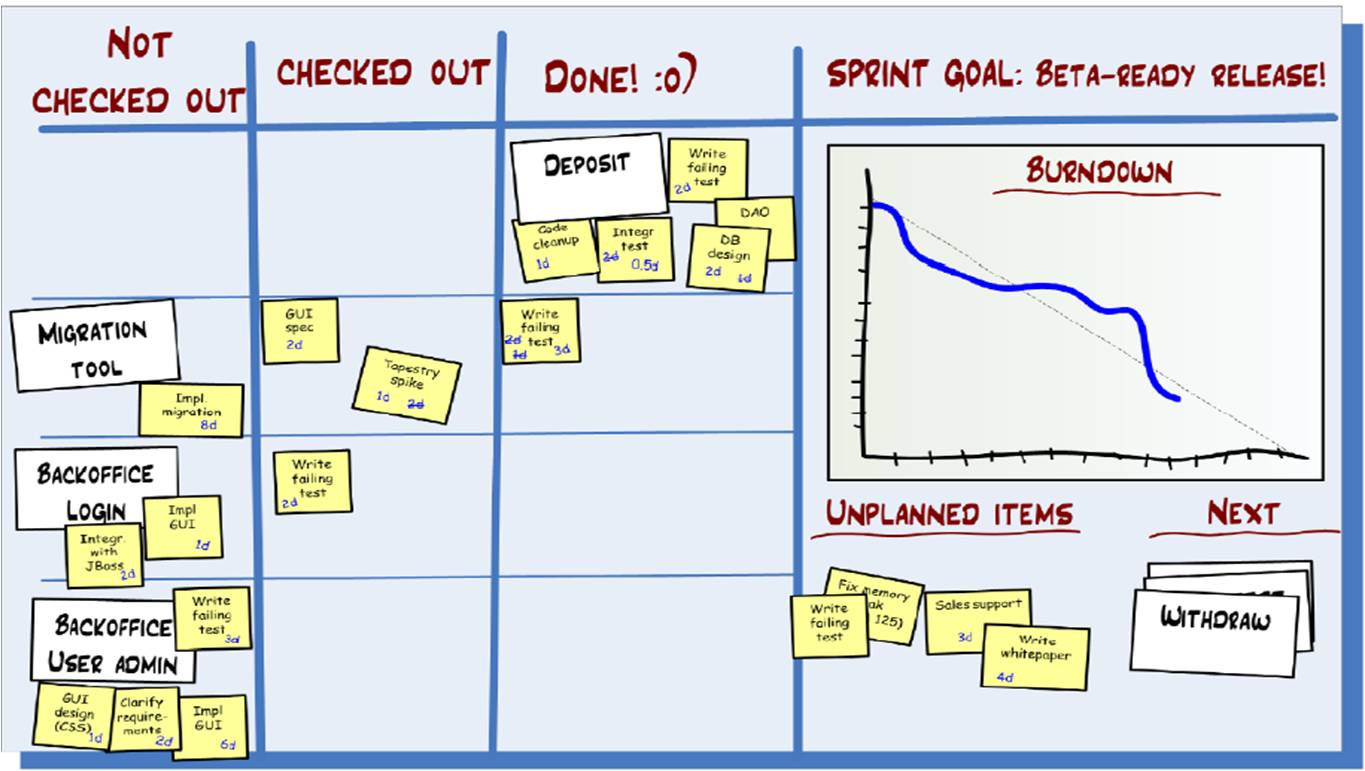
\includegraphics[width=\textwidth]{./src/img/taskboard.jpg}
\end{figureGraphics}


\subsubsection{Sprints}\label{sec:sprint}
Sprints are short development cycles, usually from one to four weeks. We were
delivering results every three weeks. During each sprint, a team creates a
shippable product, no matter how basic that product is. A sprint is composed of
a set of stories which should be completed at its end.

The interesting part of working in sprints is the idea of "making a fresh start" every three weeks. This
was quite motivating to me!


\subsection{Team}
Our team is composed of six members (me included); all software engineers with various
skills. Some are more software design oriented while others are more hardware
specialists.

Within the team, some members have a particular role:
\begin{description}
    \item[The Product owner]
        defines what the team is doing during a Sprint (see \ref{sec:sprint}).
        He determines the priority of each story (see \ref{sec:story}) the
        team is working on. His input usually comes from clients. He is the
        business-oriented person in the team. His decisions have an impact on
        the product a \gls{scrum} team delivers. Usually, he is not
        a part of the \gls{scrum} team.
    \item[The scrum master]
        ensures that every team member is correctly focused on his story. He
        keeps track of the progress of each member and alerts the
        Product owner when some impediments appear (bad time estimate of a
        story, blocking facts due to hardware, ...).
\end{description}

Note that in our team, the Product owner and the \gls{scrum} master were also contributing to the team as software engineers.
This is usually not the case since the two described roles are full-time jobs.

\subsection{Events}
In \gls{scrum}, there are several events occurring during a sprint.
These are essential to the \gls{scrum} methodology.

\subsubsection{Daily scrum}\label{sec:daily}
Every day, at 11:00 we were holding the daily \gls{scrum} meeting, also called "stand-up".
During that time, each member of the team answers quickly the three following questions:

\begin{itemize}
    \item What have I done since yesterday ?
    \item What am I planning for today ?
    \item Any issues encountered ?
\end{itemize}

This meeting is very useful, it helps tackle early problems and can assist the \gls{scrum} master to detect delays in delivering.
Note that this should not take longer than 15 minutes.


\subsubsection{Planning poker}
During planning poker sessions, we have to estimate how much time each story
would take to be done. In order to give a correct estimate, the product owner is
explaining what the exact requirements are. After that, each member of the team
should guess how much "story points" (which can sometimes be approximated to an
uninterrupted day of work) the story would take to be done. This takes place in the
form of a vote with poker session cards.

\begin{figureGraphics}{Planning poker cards}{fig:poker}
    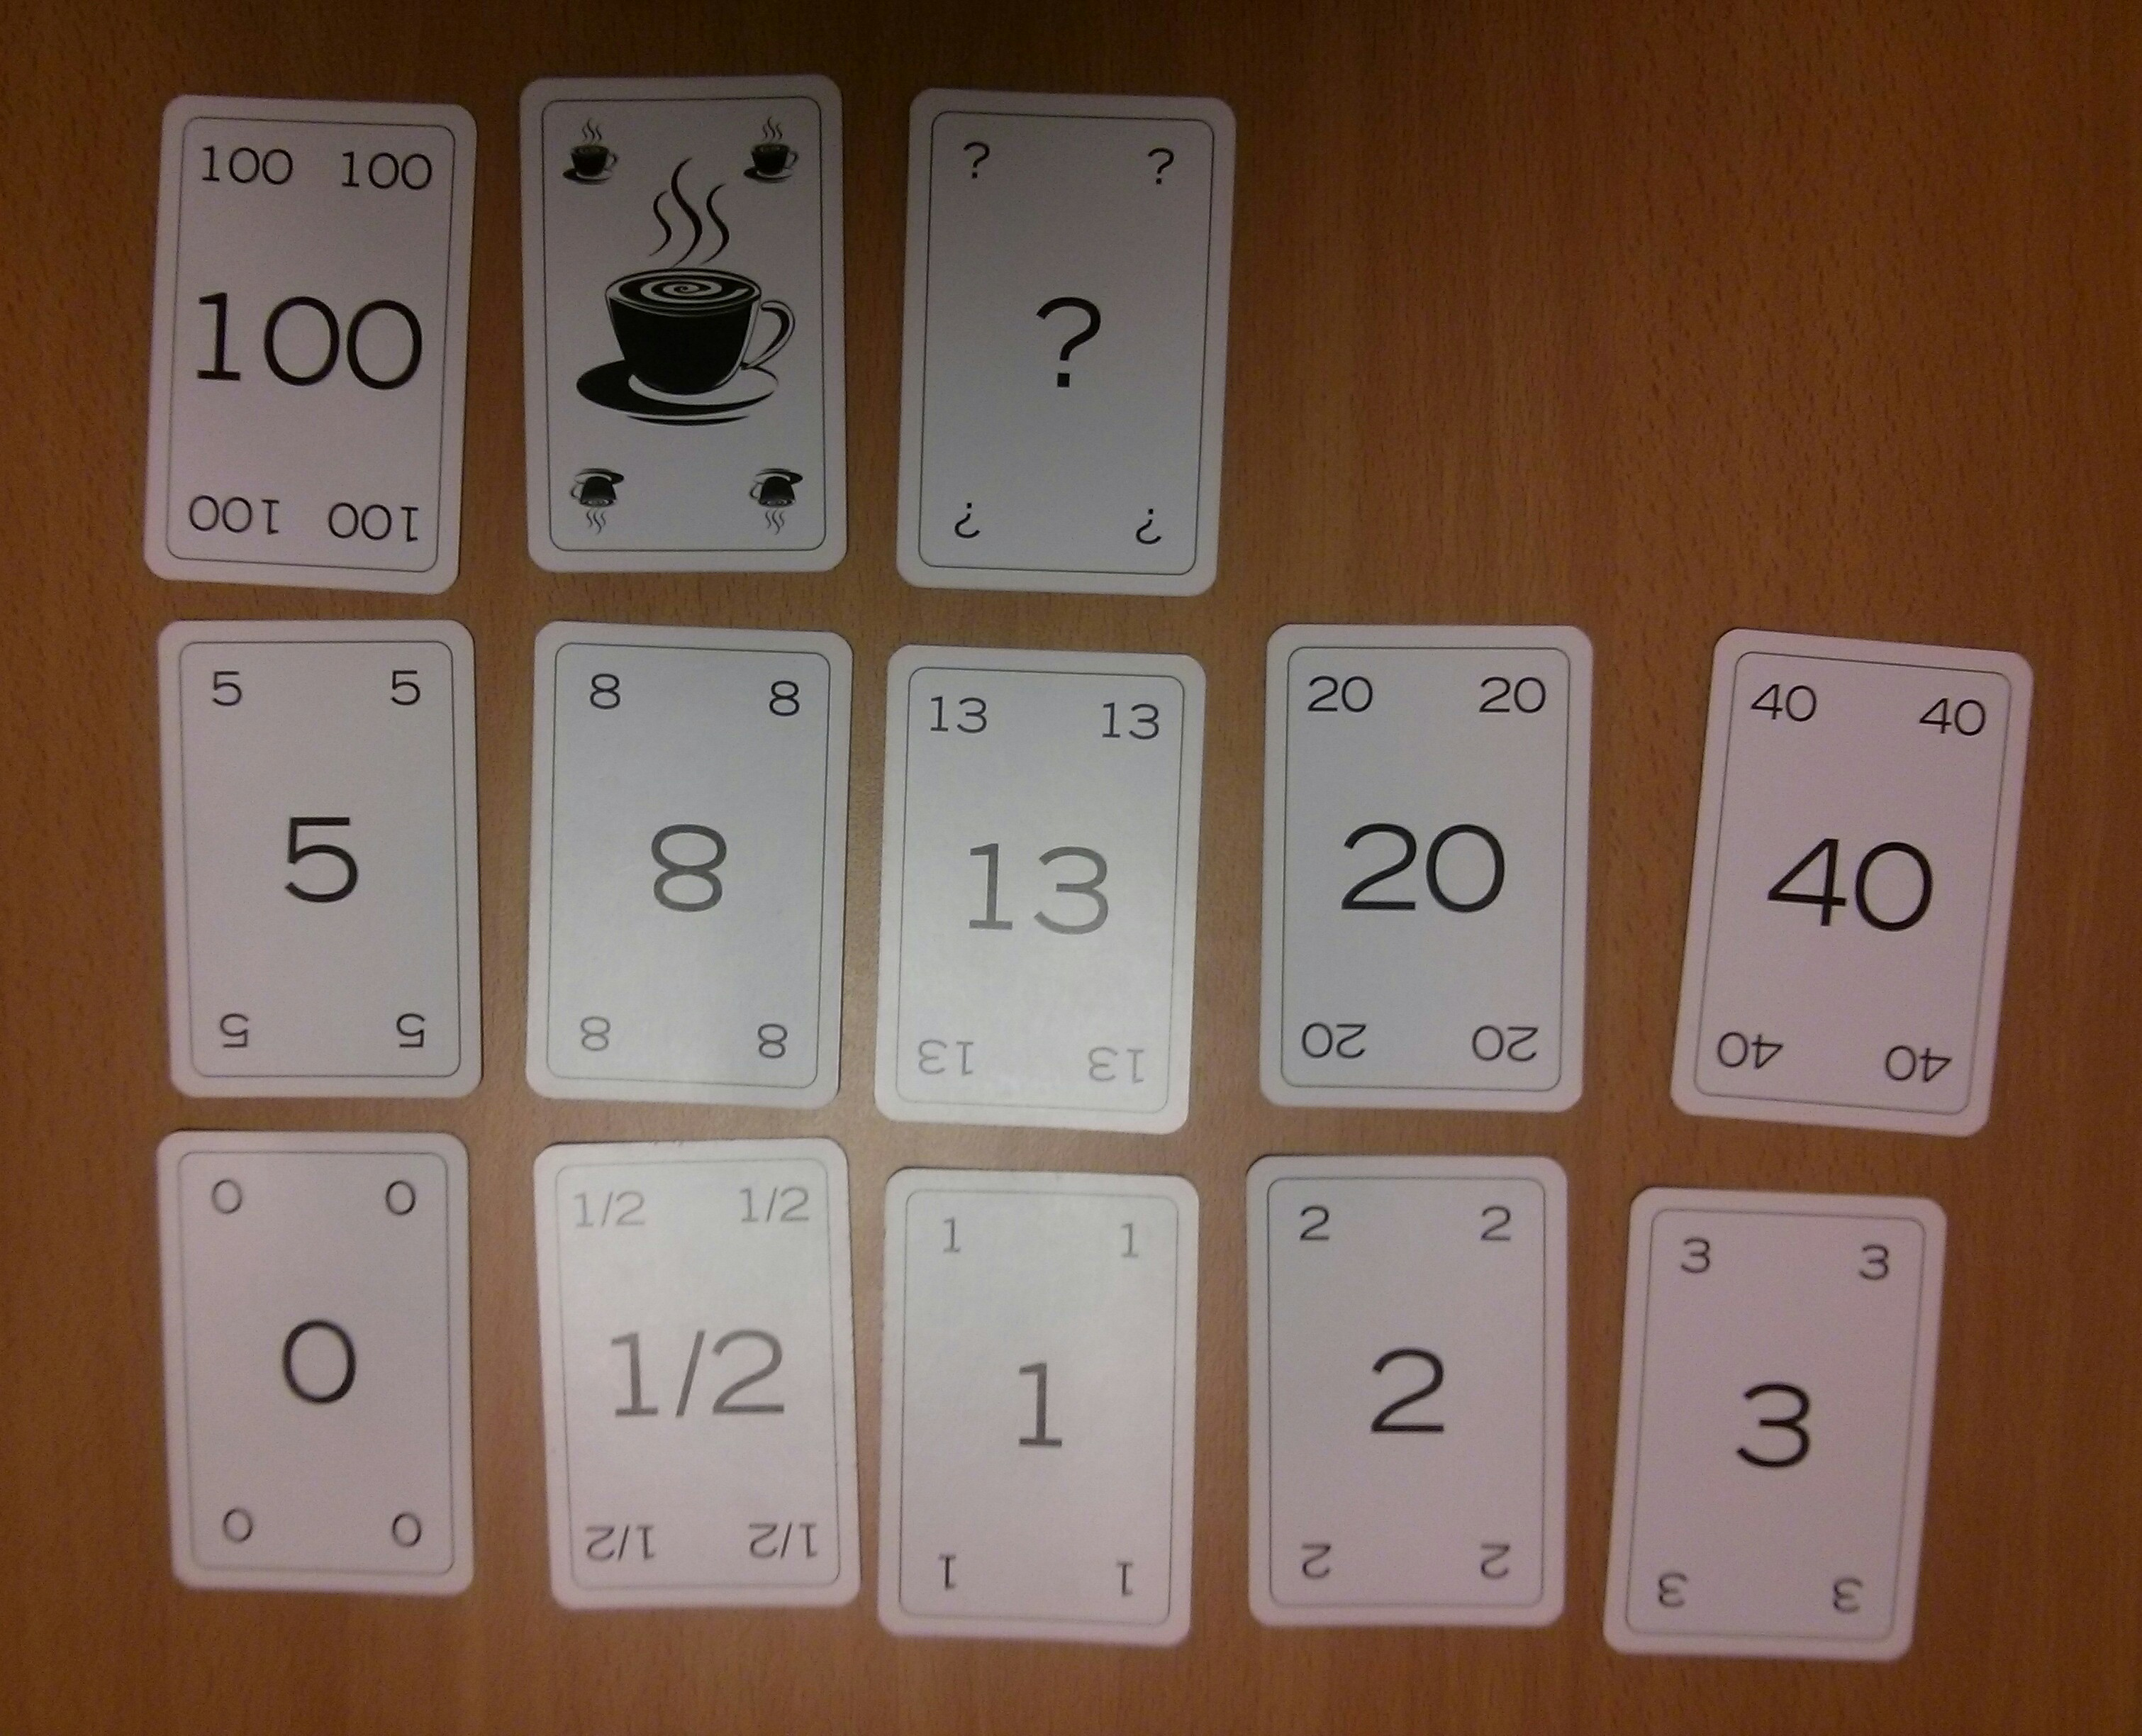
\includegraphics[width=\textwidth]{./src/img/poker.jpg}
\end{figureGraphics}

After arriving at a team consensus, the story is considered \emph{estimated}. This
is very useful so that the Product owner can prioritize the stories which have
been estimated. Rearranging a set of stories is named \emph{backlog grooming}.


\subsubsection{Demos}
At the end of each sprint, the team has to demonstrate its achievements. This
is a very important meeting with people external to the team, usually clients.
Since our development team haves no "client" in standard sense, the audience of our demos are
the integration team and the architect team.
Only the work which was \emph{done} during the last sprint is shown off during that presentation.
Work considered done is something which is \emph{shippable} and provide \emph{added value} for the customer.

This presentation is important to show the contributions that the team made.
I participated in every Demo and even showed some products since I was member of the \gls{scrum} team.

\subsubsection{Retrospectives}
After the Demo, the team has a look back at how the last sprint happened. This short meeting is made
to find out what the team did wrong last sprint, but also to highlight what the team did right.
It is frequent to see little psychological games during the retrospective, which makes all members more
eager to participate. One of the team's favorite examples, that I introduced, is the \emph{mad, sad, glad} game.

The \emph{mad, sad, glad} game happens as following:
\begin{itemize}
    \item Every team member takes 6 sticky notes
    \item For each sticky note, he must put a feeling or little sentence about
        the last sprint.
    \item Then he must put the sticky note in one of the 3 three categories: \emph{mad, sad, glad} illustrated in
        figure \ref{fig:msg}.
    \item At the end, every member must have put 2 sticky notes in each category and some items are discussed.
\end{itemize}

\begin{figureGraphics}{Mad, Sad, Glad illustration}{fig:msg}
    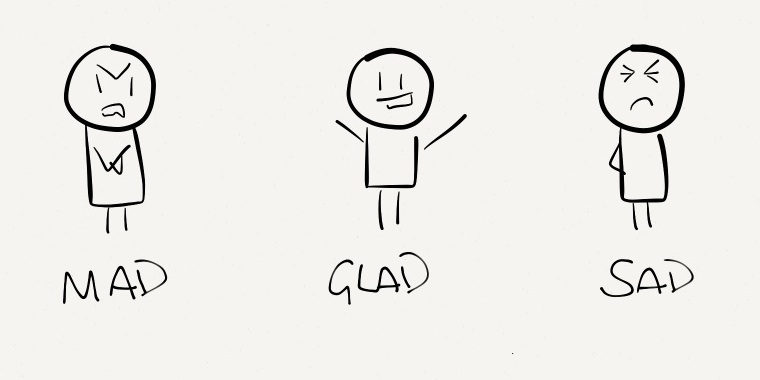
\includegraphics[height=0.2\textheight]{./src/img/mgs.png}
\end{figureGraphics}
This exercise is very popular amongst the team and we are doing it almost at every retrospective since I've introduced it.
